%\documentclass[compress]{beamer}
\documentclass[8pt]{beamer}

%-----------------------------------------------------------
% PACKAGES

%\usepackage[latin1]{inputenc}
\mode<presentation>

%\usepackage[T1]{fontenc}  
%\usetheme{Warsaw}
\usetheme{Frankfurt}

\usepackage{graphicx}
%\usepackage[section]{placeins} % force � mettre l'image o� on veut
%\usepackage{float} %utiliser H pour forcer � mettre l'image o� on veut
\usepackage{lscape} %utilisation du mode paysage
%\usepackage{pslatex}
\usepackage{url}
\usepackage{subfigure}

\usepackage{graphicx}
\usepackage{tabls}
\usepackage{afterpage}

\usepackage{ocgx2}
\usepackage[]{media9}
%\usepackage{multimedia}

\usepackage{amsthm}
\usepackage{amssymb}
\usepackage{amsmath}
\usepackage{amsfonts}
\usepackage{amstext}
\usepackage{amsbsy}
\usepackage{mathbbol} 
\usepackage{mathrsfs}

\usepackage{epsfig}
%\usepackage{epsfig}
%\usepackage{cites}
\usepackage{epsf}
\usepackage{array}
\usepackage{color}
\usepackage{pdfpages}
\usepackage{cancel}

\usepackage{tikz}
%\usepackage{booktabs}

%-----------------------------------------------------------
% NEW  DEFINITIONS
%
%=================================================================================================
% new commands
% +++++++++++++++++++++++++++++++++++++++++++++++++++++++++++++++++++++++++++++++++++++++++++++++++
\newcommand{\nc}{\newcommand}
%
% Ways of grouping things
%
\newcommand{\bracket}[1]{\left[ #1 \right]}
\newcommand{\bracet}[1]{\left\{ #1 \right\}}
\newcommand{\fn}[1]{\left( #1 \right)}
\newcommand{\ave}[1]{\left\langle #1 \right\rangle}
%
% Derivative forms
% 
\newcommand{\dx}[1]{\,d#1}
\newcommand{\dxdy}[2]{\frac{\partial #1}{\partial #2}}
\newcommand{\dxdt}[1]{\frac{\partial #1}{\partial t}}
\newcommand{\dxdz}[1]{\frac{\partial #1}{\partial z}}
\newcommand{\dfdt}[1]{\frac{\partial}{\partial t} \fn{#1}}
\newcommand{\dfdz}[1]{\frac{\partial}{\partial z} \fn{#1}}
\newcommand{\ddt}[1]{\frac{\partial}{\partial t} #1}
\newcommand{\ddz}[1]{\frac{\partial}{\partial z} #1}
\newcommand{\dd}[2]{\frac{\partial}{\partial #1} #2}
\newcommand{\ddx}[1]{\frac{\partial}{\partial x} #1}
\newcommand{\ddy}[1]{\frac{\partial}{\partial y} #1}
%
% Vector forms
%
%\renewcommand{\vec}[1]{\ensuremath{\stackrel{\rightarrow}{#1}}}
%\renewcommand{\div}{\ensuremath{\vec{\nabla} \cdot}}
%\newcommand{\grad}{\ensuremath{\vec{\nabla}}}

\renewcommand{\div}{\vec{\nabla}\! \cdot \!}
\newcommand{\grad}{\vec{\nabla}}
\newcommand{\oa}[1]{\fn{\frac{1}{3}\hat{\Omega}\!\cdot\!\overrightarrow{A_{#1}}}}

%
% Equation beginnings and endings
%
\newcommand{\bea}{\begin{eqnarray}}
\newcommand{\eea}{\end{eqnarray}}
\newcommand{\be}{\begin{equation*}}
\newcommand{\ee}{\end{equation*}}
\newcommand{\beas}{\begin{eqnarray*}}
\newcommand{\eeas}{\end{eqnarray*}}
\newcommand{\bdm}{\begin{displaymath}}
\newcommand{\edm}{\end{displaymath}}
%
% Equation punctuation
% 
\newcommand{\pec}{\hspace{0.25in},}
\newcommand{\pep}{\hspace{0.25in}.}
\newcommand{\pev}{\hspace{0.25in}}
%
% Equation labels and references, figure references, table references
% 
\newcommand{\LEQ}[1]{\label{eq:#1}}
\newcommand{\EQ}[1]{Eq.~(\ref{eq:#1})}
\newcommand{\EQS}[1]{Eqs.~(\ref{eq:#1})}
\newcommand{\REQ}[1]{\ref{eq:#1}}
\newcommand{\LFI}[1]{\label{fi:#1}}
\newcommand{\FI}[1]{Fig.~\ref{fi:#1}}
\newcommand{\RFI}[1]{\ref{fi:#1}}
\newcommand{\LTA}[1]{\label{ta:#1}}
\newcommand{\TA}[1]{Table~\ref{ta:#1}}
\newcommand{\RTA}[1]{\ref{ta:#1}}

%
% List beginnings and endings
% 
\newcommand{\bl}{\bss\begin{itemize}}
\newcommand{\el}{\vspace{-.5\baselineskip}\end{itemize}\ess}
\newcommand{\benu}{\bss\begin{enumerate}}
\newcommand{\eenu}{\vspace{-.5\baselineskip}\end{enumerate}\ess}
%
% Figure and table beginnings and endings
% 
\newcommand{\bfg}{\begin{figure}}
\newcommand{\efg}{\end{figure}}
\newcommand{\bt}{\begin{table}}
\newcommand{\et}{\end{table}}
%
% Tabular and center beginnings and endings
% 
\newcommand{\bc}{\begin{center}}
\newcommand{\ec}{\end{center}}
\newcommand{\btb}{\begin{center}\begin{tabular}}
\newcommand{\etb}{\end{tabular}\end{center}}
%
% Single space command
% 
%\newcommand{\bss}{\begin{singlespace}}
%\newcommand{\ess}{\end{singlespace}}
\newcommand{\bss}{\singlespacing}
\newcommand{\ess}{\doublespacing}
%
%---New environment "arbspace". (modeled after singlespace environment
%                                in Doublespace.sty)
%   The baselinestretch only takes effect at a size change, so do one.
% 
\def\arbspace#1{\def\baselinestretch{#1}\@normalsize}
\def\endarbspace{}
\newcommand{\bas}{\begin{arbspace}}
\newcommand{\eas}{\end{arbspace}}
%
% An explanation for a function
%
\newcommand{\explain}[1]{\mbox{\hspace{2em} #1}}
%
% Quick commands for symbols
%  
\newcommand{\half}{\frac{1}{2}}
\newcommand{\third}{\frac{1}{3}}
\newcommand{\twothird}{\frac{2}{3}}
\newcommand{\fourth}{\frac{1}{4}}
\newcommand{\mdot}{\dot{m}}
\newcommand{\ten}[1]{\times 10^{#1}\,}
\newcommand{\cL}{{\cal L}}
\newcommand{\cD}{{\cal D}}
\newcommand{\cF}{{\cal F}}
\newcommand{\cE}{{\cal E}}
\renewcommand{\Re}{\mbox{Re}}
\newcommand{\Ma}{\mbox{Ma}}
%
% Inclusion of Graphics Data
%
%\input{psfig}
%\psfiginit
%
% More Quick Commands
% 
\newcommand{\bi}{\begin{itemize}}
\newcommand{\ei}{\end{itemize}}
\newcommand{\ben}{\begin{enumerate}}
\newcommand{\een}{\end{enumerate}}
\newcommand{\dxi}{\Delta x_i}
\newcommand{\dyj}{\Delta y_j}
\newcommand{\ts}[1]{\textstyle #1}


\newcommand{\bu}{\boldsymbol{u}}
\newcommand{\ber}{\boldsymbol{e}}
\newcommand{\br}{\boldsymbol{r}} 
\newcommand{\bo}{\boldsymbol{\Omega}}

\newcommand{\bn}{\boldsymbol{\nabla}}

% DGFEM commands
\newcommand{\jmp}[1]{[\![#1]\!]}                     % jump
\newcommand{\mvl}[1]{\{\!\!\{#1\}\!\!\}}             % mean value


\newcommand{\boxedeqn}[1]{%
  \[\fbox{%
      \addtolength{\linewidth}{-2\fboxsep}%
      \addtolength{\linewidth}{-2\fboxrule}%
      \begin{minipage}{\linewidth}%
      \begin{equation}#1\end{equation}%
      \end{minipage}%
    }\]%
}
\newcommand{\mboxed}[1]{\boxed{\phantom{#1}}}
\newcommand{\ud}{\,\mathrm{d}}

% keff
\newcommand{\keff}{\ensuremath{k_{\textit{eff}}}}

% margin par
\newcommand{\mt}[1]{\marginpar{ {\footnotesize #1} }}

% shortcut for aposterio in italics
\newcommand{\apost}{\textit{a posteriori\xspace}}
\newcommand{\Apost}{\textit{A posteriori}\xspace}

% shortcut for multi-group
\newcommand{\mg}{multigroup\xspace}
\newcommand{\Mg}{Multigroup\xspace}
\newcommand{\ho}{higher-order\xspace}
\newcommand{\Ho}{Higher-order\xspace}
\newcommand{\HO}{Higher-Order\xspace}
\newcommand{\HObig}{HIGHER-ORDER\xspace}
\newcommand{\Mgbig}{MULTIGROUP\xspace}

% shortcut for domain notation
\newcommand{\D}{\mathcal{D}}

% shortcut for xuthus
\newcommand{\psc}[1]{{\sc {#1}}}
\newcommand{\xuthus}{\psc{xuthus}\xspace}

% vector shortcuts
\newcommand{\vo}{\vec{\Omega}}
\newcommand{\vr}{\vec{r}}
\newcommand{\vn}{\vec{n}}
\newcommand{\vnk}{\vec{\mathbf{n}}}

% extra space
\newcommand{\qq}{\quad\quad}

% sign function
\DeclareMathOperator{\sgn}{sgn}


\newcommand{\ensuretext}[1]{\ensuremath{\text{#1}}}

% common reference commands
\newcommand{\eqt}[1]{Eq.~(\ref{#1})}                     % equation
\newcommand{\fig}[1]{Fig.~\ref{#1}}                      % figure
\newcommand{\tbl}[1]{Table~\ref{#1}}                     % table



\newcommand{\rhs}{right-hand-side\xspace}
\newcommand{\clearemptydoublepage}{\newpage{\pagestyle{empty}\cleardoublepage}}


\newcommand{\bs}[1]{\mathbf{#1}}
\renewcommand{\bs}[1]{\vec{#1}}
%\newcommand{\dd}{\mathrm{d}}
\newcommand{\norm}[1]{\left\lVert#1\right\rVert_{L^2}}
\renewcommand{\Re}{\textrm{Re}}
\newcommand{\Pe}{\textrm{P\'e}}
\renewcommand{\Pr}{\textrm{Pr}}

\newcommand{\resi}{R_e}
%\newcommand{\resinew}{\tilde{D}_e}
\newcommand{\resinew}{\widetilde{\resi}}
\newcommand{\matder}[1]{\frac{\textrm{D} #1}{\textrm{D} t}}

\newcommand{\divv}[1]{\vec{\nabla}^{#1}\! \cdot \!}
\newcommand{\gradd}[1]{\vec{\nabla}^{#1}}

\newcommand{\tcr}[1]{\textcolor{red}{#1}}
\newcommand{\tcb}[1]{\textcolor{blue}{#1}}
\newcommand{\tcm}[1]{\textcolor{magenta}{#1}}
\newcommand{\tcp}[1]{\textcolor{violet}{#1}}

\renewcommand{\L}{\mathbf{L}}
\renewcommand{\S}{\mathbf{\Sigma}}
\newcommand{\M}{\mathbf{M}}
\renewcommand{\D}{\mathbf{D}}

% tikz stuff
\usetikzlibrary{shapes,arrows,positioning}
\pgfdeclarelayer{background}
\pgfdeclarelayer{foreground}
\pgfsetlayers{background,main,foreground}
\tikzstyle{redblock}=[rectangle, draw, align=center, top color=red!25, bottom color=red!75,  minimum width=10mm, minimum height=10mm,]
\tikzstyle{blueblock}=[rectangle,draw, align=center, top color=blue!25, bottom color=blue!75,  minimum width=10mm, minimum height=10mm]
\tikzstyle{purpleblock}=[rectangle,  draw, align=center, top color=purple!25, bottom color=purple!75, minimum width=10mm, minimum height=10mm]
\tikzstyle{orangeblock}=[rectangle, draw, align=center, top color=orange!25, bottom color=orange!75,  minimum width=10mm, minimum height=10mm]
\tikzstyle{greendiamond}=[diamond, draw, align=center, top color=green!25, bottom color=green!75,  minimum width=8mm, aspect=2]

%=================================================================================================

%============================================================

%style et couleur
%\usetheme{Frankfurt}
\date{\today}

%\addtobeamertemplate{footline}{\hfill\insertframenumber/\inserttotalframenumber\hspace{2em}\null}

\setbeamertemplate{footline}{
\leavevmode%
%\hbox{\hspace*{-0.06cm}
\begin{beamercolorbox}[wd=.5\paperwidth,ht=3.25ex,dp=1ex,center]{author in head/foot}%
	\usebeamerfont{author in head/foot}\insertshortauthor%~~(\insertshortinstitute)
\end{beamercolorbox}%
\begin{beamercolorbox}[wd=.25\paperwidth,ht=3.25ex,dp=1ex,center]{section in head/foot}%
	\usebeamerfont{section in head/foot} IQS PHYSOR 2016 % \insertshorttitle
\end{beamercolorbox}%
\begin{beamercolorbox}[wd=.25\paperwidth,ht=3.25ex,dp=1ex,left]{section in head/foot}%
	\usebeamerfont{section in head/foot}\insertshortdate{}\hspace*{2em}
	\insertframenumber{} / \inserttotalframenumber %\hspace*{2ex}
\end{beamercolorbox}}%
%\vskip0pt%
%}

\beamertemplatetransparentcovered

\urldef{\ragusa}\url{jean.ragusa@tamu.edu}
\urldef{\prince}\url{zachmprince@tamu.edu}

\title{Improved Quasi-Static Method in Rattlesnake}

\author{Zachary M. Prince, Jean C. Ragusa}
\institute{Department of Nuclear Engineering, Texas A\&M University, College Station, TX}

%%%%%%%%%%%%%%%%%%%%%%%%%%%%%%%%%%%%%%%%%%%%%%%%%%%%%%%%%%%%%%%%%%%%

%%%%%%%%%%%%%%%%%%%%%%%%%%%%%%%%%%%%%%%%%%%%%%%%%%%%%%%%%%%%%%%%%%%%
%%%%%%%%%%%%%%%%%%%%%%%%%%%%%%%%%%%%%%%%%%%%%%%%%%%%%%%%%%%%%%%%%%%%
\begin{document}
%%%%%%%%%%%%%%%%%%%%%%%%%%%%%%%%%%%%%%%%%%%%%%%%%%%%%%%%%%%%%%%%%%%%
%%%%%%%%%%%%%%%%%%%%%%%%%%%%%%%%%%%%%%%%%%%%%%%%%%%%%%%%%%%%%%%%%%%%

%-------------------------------------------------------------------
\begin{frame}
%\vspace{-1.5cm}
	\begin{figure}[t]
		\centering
			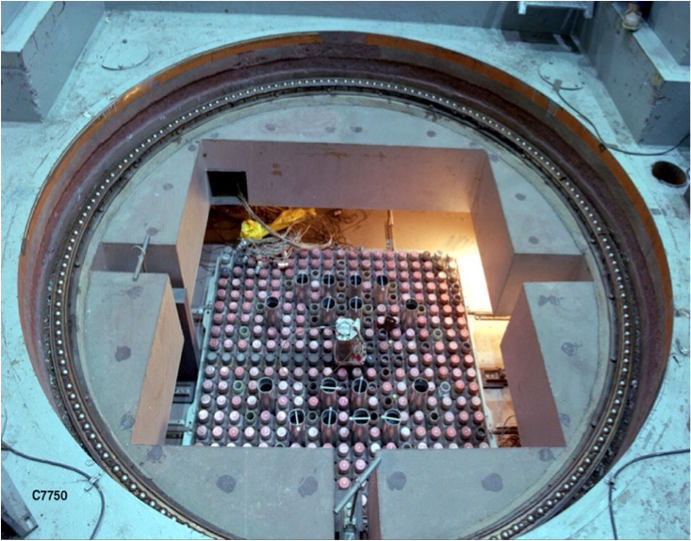
\includegraphics[width=.45\textwidth]{figures/Treat_core_view.png}
	\end{figure}
\vspace{-0.5cm}
\titlepage
\vspace{-0.5cm}
\small{email: {\prince} }

\end{frame}
%-------------------------------------------------------------------

%-------------------------------------------------------------------
\begin{frame}
	\frametitle{Outline}
	\tableofcontents 
\end{frame}
%-------------------------------------------------------------------

%%%%%%%%%%%%%%%%%%%%%%%%%%%%%%%%%%%%%%%%%%%%%%%%%%%%%%%%%%%%%%%%%%%%
%%%%%%%%%%%%%%%%%%%%%%%%%%%%%%%%%%%%%%%%%%%%%%%%%%%%%%%%%%%%%%%%%%%%
\section{IQS Theory}
%%%%%%%%%%%%%%%%%%%%%%%%%%%%%%%%%%%%%%%%%%%%%%%%%%%%%%%%%%%%%%%%%%%%
%%%%%%%%%%%%%%%%%%%%%%%%%%%%%%%%%%%%%%%%%%%%%%%%%%%%%%%%%%%%%%%%%%%%

%%%%%%%%%%%%%%%%%%%%%%%%%%%%%%%%%%%%%%%%%%%%%%%%%%%%%%%%%%%%%%%%%%%%
\subsection{Time-dependent Multigroup Diffusion}
%%%%%%%%%%%%%%%%%%%%%%%%%%%%%%%%%%%%%%%%%%%%%%%%%%%%%%%%%%%%%%%%%%%%

%-------------------------------------------------------------------
\begin{frame}{Time-dependent Multigroup Diffusion}

\vspace{-3mm}

\begin{block}{Group Fluxes $\phi^g$ $(1 \le g \le G )$ with Precursors $C_i$ $(1 \le i \le I)$}
\begin{align*}
\frac{1}{v^g} \frac{\partial \phi^g }{\partial t} =& \frac{\chi_p^g}{\keff} \sum_{g'=1}^G (1-\beta) \nu^{g'} \Sigma_f^{g'} \phi^{g'} -  \left( -\div D^g \grad  + \Sigma_r^g \right) \phi^g  \nonumber \\
&  + \sum_{g'\neq g}^G\Sigma_s^{g'\to g} \phi^{g'}  + \sum_{i=1}^I\chi_{d,i}^g\lambda_i C_i \ , \quad 1 \le g \le G 
\end{align*}
\be
\frac{dC_i}{dt} = \frac{\beta_i}{k_{eff}}\sum_{g=1}^G\nu^{g} \Sigma_f^g \phi^{g} - \lambda_i C_i \ , \quad 1 \le i \le I 
\ee
\end{block}

%\vspace{-4mm}

\begin{block}{Flux Factorization}
Decomposition of the multigroup flux into the product of a time-dependent \tcr{amplitude} ($\tcr{p}$) and a space-/time-dependent multigroup \tcb{shape} ($\tcb{\varphi^g}$):
\begin{equation*}
\phi^g(\vec{r},t) = \tcr{p(t)} \tcb{\varphi^g(\vec{r},t)}
\end{equation*}

\begin{itemize}
\item 
Factorization is \textbf{not} an approximation.
\item
Note that $\tcr{p(t)}$ and $\tcb{\varphi^g(\vec{r},t)}$ are not unique. 
%\[
%\phi= \tcr{p} \times \tcb{\psi} = \tcr{\frac{p}{a}} \times \tcb{\left( a \psi \right)}
%\]
\end{itemize}
\end{block}
%--------------

\end{frame}
%-------------------------------------------------------------------


%%%%%%%%%%%%%%%%%%%%%%%%%%%%%%%%%%%%%%%%%%%%%%%%%%%%%%%%%%%%%%%%%%%%
\subsection{IQS Equations}
%%%%%%%%%%%%%%%%%%%%%%%%%%%%%%%%%%%%%%%%%%%%%%%%%%%%%%%%%%%%%%%%%%%%

%-------------------------------------------------------------------
\begin{frame}{Shape equations}

\begin{block}{Shape equations}
Implementing factorization and solving for $\tcb{\varphi^g}$:
\begin{align*}
\frac{1}{v^g} \frac{\partial \tcb{\varphi^g} }{\partial t} =& \frac{\chi_p^g}{\keff} \sum_{g'=1}^G (1-\beta) \nu^{g'} \Sigma_f^{g'} \tcb{\varphi^{g'}} -  \left( -\div D^g \grad  + \Sigma_r^g + \tcr{\frac{1}{v^g}}\tcr{\frac{1}{p}}\tcr{\frac{dp}{dt}}\right) \tcb{\varphi^g}  \nonumber \\
&  + \sum_{g'\neq g}^G\Sigma_s^{g'\to g} \tcb{\varphi^{g'}}  + \tcr{\frac{1}{p}}\sum_{i=1}^I\chi_{d,i}^g\lambda_i C_i \ , \quad 1 \le g \le G 
\end{align*}
\begin{equation*}
\frac{dC_i}{dt} = \tcr{p}\sum_{g=1}^G \nu_{d,i} \Sigma_f^g \tcb{\varphi^{g}} - \lambda_iC_i , \quad 1 \le i \le I
\end{equation*}
%\be
%\frac{dC_i}{dt} = \frac{\beta_i}{k_{eff}}\sum_{g=1}^G\nu^{g} \Sigma_f^g \tcr{p} \varphi^{g} - \lambda_i C_i \ , \quad 1 \le i \le I 
%\ee
\end{block}

\begin{block}{Differences with original transport equation}
\ben
\item An additional removal term based on $\tcr{\frac{1}{v^g}\frac{1}{p}\frac{dp}{dt}} \tcb{\psi^g}$
\item Delayed neutron source term scaled by $\tcr{\frac{1}{p}}$
\item The delayed fission source in the precursor equation scaled by \tcr{p}
\een
\end{block}

\end{frame}
%-------------------------------------------------------------------

%%%%%%%%%%%%%%%%%%%%%%%%%%%%%%%%%%%%%%%%%%%%%%%%%%%%%%%%%%%%%%%%%%%%
% \subsection{Amplitude equations}
%%%%%%%%%%%%%%%%%%%%%%%%%%%%%%%%%%%%%%%%%%%%%%%%%%%%%%%%%%%%%%%%%%%%


%-------------------------------------------------------------------
\begin{frame}{Amplitude equations (PRKE)}

\begin{block}{Principle}
To obtain the \tcr{amplitude} equation, we multiply the shape equations with a weighting 
function (initial adjoint flux, $\phi^{*g}$), then integrate over domain.  
\end{block}

\begin{block}{Notation}
For brevity, the adjoint flux product and integration over domain will be represented with parenthetical notation:
\[
\int_D\phi^{*g}(\vec{r})f(\vec{r})dr^3=\left(\phi^{*g},f\right)
\]
\end{block}


\begin{block}{Uniqueness of the factorization}
In order to impose uniqueness of the factorization, one requires:
\[
\tcp{K_0} = \sum_{g=1}^G\left(\phi^{*g},\frac{1}{v^g}\varphi^g\right)= constant
\]
\tcm{This condition will be the criteria for solution convergence}
\end{block}


\end{frame}
%-------------------------------------------------------------------

%-------------------------------------------------------------------
\begin{frame}{Point Reactor Kinetics Equation}
\vspace{-2mm}
\begin{block}{PRKE}
\[
\frac{d\tcr{p}}{dt}=\left[\frac{\rho-\bar{\beta}}{\Lambda}\right]\tcr{p}+\sum_{i=1}^I\bar{\lambda}_i\xi_i
\]
\[
\frac{d\xi_i}{dt}=\frac{\bar{\beta}_i}{\Lambda}\tcr{p} - \bar{\lambda}_i\xi_i \quad 1 \le i \le I 
\]
\end{block}
%\vspace{-3mm}
\begin{block}{PRKE Coefficients}

\small \be
\frac{\rho-\bar{\beta}}{\Lambda}=
\frac{ \sum_{g=1}^G \left(\phi^{*g},\sum_{g'=1}^G\frac{\chi_p^g}{\keff} \nu_p^{g'} \Sigma_f^{g'}\varphi^{g'} + \sum_{g'\neq g}^G\Sigma_s^{g'\to g} \varphi^{g'} -\left( -\div D^g \grad  + \Sigma_r^g \right)\varphi^g\right)}
{\sum_{g=1}^G \left(\phi^{*g},\frac{1}{v^g}\varphi^g\right)}
\ee \normalsize
%%
\be
\frac{\bar{\beta}}{\Lambda}=\sum_{i=1}^I\frac{\bar{\beta}_i}{\Lambda}=\frac{1}{\keff}
\frac{\sum_{i=1}^I\sum_{g=1}^G(\phi^{*g}, \beta_i\nu^{g} \Sigma_f^g \varphi^{g})}
{\sum_{g=1}^G \left(\phi^{*g},\frac{1}{v^g}\varphi^g\right)}
\ee
%%
\be
\bar{\lambda}_i=\frac{\sum_{g=1}^G(\phi^{*g},\chi_{d,i}^g\lambda_i C_i)}{\sum_{g=1}^G(\phi^{*g},\chi_{d,i}^gC_i)}
\ee

\end{block}

\end{frame}
%-------------------------------------------------------------------

%-------------------------------------------------------------------
%\begin{frame}{Shape equations: Implementation within the MOOSE framework}
%
%\begin{block}{Shape equations $\to$ \tcm{FEM solver + implicit time integration}}
%\begin{equation*}
%\boxed{
%\frac{1}{v}\frac{\tcb{\psi}^{n+1}-\tcb{\psi}^n }{\Delta t} = \left(H^{n+1} + P_p^{n+1} - L^{n+1} -\tcr{\frac{1}{v}\frac{1}{p^{n+1}}\left.\frac{dp}{dt}\right|_{n+1}} \right) \tcb{\psi}^{n+1}  + \tcr{\frac{1}{p^{n+1}}} S_{d}^{n+1} 
%}
%\end{equation*}
%\end{block}
%
%\begin{block}{Modification to the original transport equation}
%\ben
%\item An additional removal term based on $\tcr{\frac{1}{v^g}\frac{1}{p}\frac{dp}{dt}} \tcb{\psi^g}$\\
%\tcm{$\to$ add a new kernel in Rattlesnake} (easy)
%\item Delayed neutron source term scaled by $\tcr{\frac{1}{p}}$\\
%\tcm{$\to$ scale the delayed neutron source kernel} (easy)
%\item nonlinear coupling between shape variable $\tcb{\psi^{n+1}}$ and amplitude variable $\tcr{p^{n+1}}$\\
%\tcm{$\to$ employ MOOSE's nonlinear solvers} (easy)
%\een
%\end{block}
%
%\end{frame}
%-------------------------------------------------------------------


%%%%%%%%%%%%%%%%%%%%%%%%%%%%%%%%%%%%%%%%%%%%%%%%%%%%%%%%%%%%%%%%%%%%
\subsection{IQS method solution process}
%%%%%%%%%%%%%%%%%%%%%%%%%%%%%%%%%%%%%%%%%%%%%%%%%%%%%%%%%%%%%%%%%%%%

%-------------------------------------------------------------------
\begin{frame}{IQS}

\begin{block}{Factorization leads to a nonlinear system}
The \tcr{amplitude} and \tcb{shape} equations form a system of nonlinear coupled equations: 
\ben
\item the coefficients appearing in the \tcr{PRKE}'s depend upon the \tcb{shape} solution,
\item the \tcb{shape} equation has a kernel dependent on \tcr{amplitude} and its derivative,  
%\item the delayed neutron source term is scaled by the amplitude.
\een
\end{block}

\begin{block}{Time scales and IQS method solution process}
Because solving for the \tcb{shape} can be expensive, especially in two or three dimensions, it is attractive to make the assumption that the \tcb{shape} is weakly time-dependent so the \tcb{shape} can be computed after a multitude of \tcr{PRKE} calculations:
%

\begin{figure}[h]
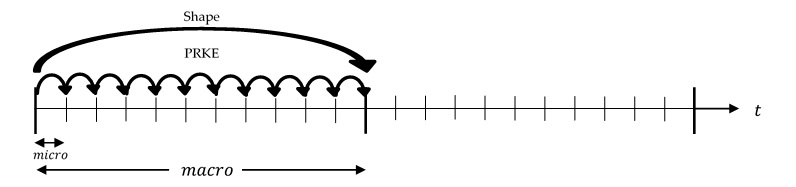
\includegraphics[width=\linewidth]{figures/IQS_visualization.jpg}
%\caption{IQS method solution process}
\label{fig:IQS}
\end{figure}

\tcm{Currently, in MOOSE, we employ the available Picard iteration functionality to resolve the nonlinearities. Later, nonlinearities will also be resolved using Newton iteration.}
\end{block}
\end{frame}
%-------------------------------------------------------------------

%-------------------------------------------------------------------
\begin{frame}{Convergence criteria}


\begin{block}{Ideally}
The normalization constant should not change over time !
\[
\tcp{K_0} = \sum_{g=1}^G\left(\phi^{*g},\frac{1}{v^g}\varphi^g_0\right)= constant
\]
\[
\text{Thus, we employ }\quad
\left| \frac{\sum_{g=1}^G\left(\phi^{*g},\frac{1}{v^g}\varphi^g_{n+1}\right)}{\tcp{K_0}}-1\right| 
= \left| \frac{\tcp{K_{n+1}}}{{\tcp{K_0}}}-1\right|  < tol
\]
\end{block}

\begin{block}{Note that we have seen in practice ... }
\[
\frac{ \| \varphi^{g,\tcr{\ell+1}}_{n+1} - \varphi^{g,\tcr{\ell}}_{n+1} \|}{\| \varphi^{g,\tcr{\ell+1}}_{n+1} \|} < tol 
\quad \text{or even} \quad
\frac{ \| \varphi^{g,\tcr{\ell+1}}_{n+1} - \varphi^{g,\tcr{0}}_{n+1} \|}{\| \varphi^{g,\tcr{0}}_{n+1} \|} < tol 
\]
where $\tcr{\ell}$ is the IQS iteration index over a given macro time step $[t_n,t_{n+1}]$\\
\smallskip
These empirical criteria must be followed by a renormalization before starting the next time step $[t_{n+1},t_{n+2}]$
\[
 \varphi^{g,\tcr{converged}}_{n+1} \times \frac{\tcp{K_{n+1}^{\tcr{converged}}}}{\tcp{K_0}} \rightarrow \varphi^{g}_{n+1}
\]
\end{block}


\end{frame}
%-------------------------------------------------------------------

%-------------------------------------------------------------------
\begin{frame}{IQS Predictor-Corrector}

%\begin{block}{IQS P-C Linearizes the System}
IQS P-C linearizes the system and avoids iterations on the \tcb{shape}: 
\ben
\item Evaluate multigroup diffusion equation to get predicted flux $\phi_{n+1}^{g,\tcr{pred}}$
\item Scale predicted flux to obtain \tcb{shape}:
\[
\tcb{\varphi^{g}_{n+1}} = \phi_{n+1}^{g,\tcr{pred}} \frac{\sum_{g=1}^G\left(\phi^{*g},\frac{1}{v^g}\varphi^g_{n+1}\right)}{\sum_{g=1}^G \left(\phi^{*g},\frac{1}{v^g}\phi_{n+1}^{g,\tcr{pred}}\right)} = \phi_{n+1}^{g,\tcr{pred}} \frac{\tcp{K_0}}{\tcp{K_{n+1}}}
\]
\item Compute PRKE parameters at $t_{n+1}$
\item Evaluate PRKE along micro step using interpolated parameters to obtain $\tcr{p_{n+1}}$
\item Scale $\tcb{\varphi^{g}_{n+1}}$ to obtain corrected flux:
\[
\phi_{n+1}^{g,\tcr{corr}} = \tcr{p_{n+1}} \times \tcb{\varphi^{g}_{n+1}}
\]
\een

 Advantage: No IQS nonlinear iteration is necessary \\
 Disadvantage: Assumes $\sum_{g=1}^G\left(\phi^{*g},\frac{1}{v^g}\varphi^g_{n+1}\right)$ is inherently constant \\
\vspace{2mm}
\small \tcm{Note: The PRKE parameters can be computed using flux since the amplitude is in the numerator and denominator of each one. So Step 2 is unnecessary if the corrected flux is solved with}:
\[
\phi_{n+1}^{g,\tcr{corr}} = \phi_{n+1}^{g,\tcr{pred}} \times \frac{\tcp{K_0}}{\tcp{K_{n+1}}} \tcr{p_{n+1}}
\]
\normalsize
%\end{block}

\end{frame}
%-------------------------------------------------------------------

%%%%%%%%%%%%%%%%%%%%%%%%%%%%%%%%%%%%%%%%%%%%%%%%%%%%%%%%%%%%%%%%%%%%
%%%%%%%%%%%%%%%%%%%%%%%%%%%%%%%%%%%%%%%%%%%%%%%%%%%%%%%%%%%%%%%%%%%%
\section{Step Doubling}
%%%%%%%%%%%%%%%%%%%%%%%%%%%%%%%%%%%%%%%%%%%%%%%%%%%%%%%%%%%%%%%%%%%%
%%%%%%%%%%%%%%%%%%%%%%%%%%%%%%%%%%%%%%%%%%%%%%%%%%%%%%%%%%%%%%%%%%%%

\subsection{Theory}

%-------------------------------------------------------------------
\begin{frame}{Theory}

\begin{block}{Motivation}
\begin{itemize}
\item The concept of time adaptation is to have the behavior of some aspect of the evaluation determine the size of the time step.
\item The computational efficiency of IQS is best demonstrated when time adaptation is applied.
\item Step doubling adaptation was chosen because it is relatively simple and it utilizes the behavior of the solution to determine step size.
\end{itemize}
\end{block}

\begin{block}{Local Truncation Error}
We can estimate the local truncation error of the latest solve with a Taylor series expansion:
\be
\norm{LTE_n} = \Delta t_n^{p+1} \norm{\frac{y^{p+1}_{n-1}}{(p+1)!} + \Delta t_n \frac{y^{p+2}_{n-1}}{(p+2)!} + ...}
\ee
Where $p$ is the time discretization method's order and $y_n$ is the solution at time $ = t_n$. $\Delta t_n$ was the latest solves time step and $\Delta t_{n+1}$ is the next solves time step that has a desired error $\norm{LTE_{n+1}}$.  It can be

\end{block}

\end{frame}
%-------------------------------------------------------------------


%-------------------------------------------------------------------
\begin{frame}{Theory}

\begin{block}{New Step Size}
Using the definitions of the local errors:
\be
\Delta t_{n+1}^{p+1} \simeq \Delta t_{n}^{p+1} \theta \frac{\norm{LTE_{n+1}}}{\norm{LTE_{n}}}
\ee
Where $\theta \equiv 1 + O(\Delta t_n)$. $\norm{LTE_{n+1}}$ is some user defined relative error tolerance ($e_{tol}$) and $\delta_n \equiv \frac{\theta}{\norm{LTE_{n}}}$ is a method's approximation to the last step's local error ($e_n$).  Therefore in practice:
\be
\Delta t_{new} = \Delta t_{old} \left[\frac{e_{tol}}{e_n}\right]^{1/(p+1)}
\ee
\end{block}

\begin{block}{Step Doubling}
Step doubling approximates the local error ($\delta_n$) by taking the difference in the local error of a solution with $\Delta t$ ($y_{\Delta t}$) and $\Delta t/2$ ($y_{\Delta t/2}$):
\be
e_n = \frac{\norm{y_{\Delta t/2} - y_{\Delta t}}}{\text{max}\left(\norm{y_{\Delta t/2}},\norm{y_{\Delta t}}\right)}
\ee
\end{block}

\end{frame}
%-------------------------------------------------------------------

\subsection{Solution Process}

%-------------------------------------------------------------------
\begin{frame}{Solution Process}

\begin{block}{Solution Process with IQS}
\begin{figure}[htpb!]
\centering
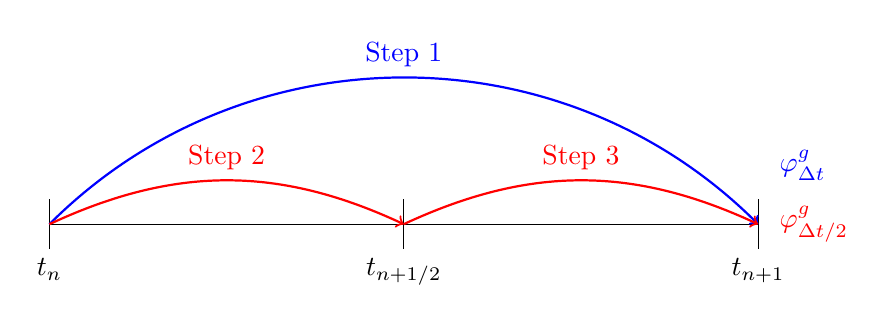
\begin{tikzpicture}[scale=1.5]
\draw[] (0,2) -- (6,2) ;
\foreach \x in  {0,3,6}
\draw[shift={(\x,2)},color=black] (0pt,6pt) -- (0pt,-6pt);
\draw[shift={(0,2)},color=black] (0pt,0pt) -- (0pt,-6pt) node[below] {$t_n$};
\draw[shift={(3,2)},color=black] (0pt,0pt) -- (0pt,-6pt) node[below] {$t_{n+1/2}$};
\draw[shift={(6,2)},color=black] (0pt,0pt) -- (0pt,-6pt) node[below] {$t_{n+1}$};
\draw (0,2) edge[out=45,in=135,->,thick,blue] node[above,sloped] {\tcb{Step 1}} (6,2);
\draw (0,2) edge[out=25,in=155,->,thick,red] node[above,sloped] {\tcr{Step 2}} (3,2);
\draw (3,2) edge[out=25,in=155,->,thick,red] node[above,sloped] {\tcr{Step 3}} (6,2);
\node[anchor=west](shape) at (6.1,2.5) {$\tcb{\varphi_{\Delta t}^g}$};
\node[anchor=west](shape) at (6.1,2) {$\tcr{\varphi_{\Delta t/2}^g}$};

\end{tikzpicture}
\end{figure}
\be
e_n =\frac{\norm{\sum_{g=1}^G \left(\tcr{\varphi^g_{\Delta t/2}} - \tcb{\varphi^g_{\Delta t}} \right)}}{\max\left(\norm{\sum_{g=1}^G\tcr{\varphi^g_{\Delta t/2}}},\norm{\sum_{g=1}^G\tcb{\varphi^g_{\Delta t}}}\right)} 
\qq  \qq 
\Delta t_{new} = S_f \Delta t \left[\frac{e_{tol}}{e_n}\right]^{1/(p+1)}   
\ee

\end{block}
\end{frame}
%-------------------------------------------------------------------

%-------------------------------------------------------------------
\begin{frame}{Solution Process}
\begin{block}{Programming Visualization}
\begin{figure}[!htpb]
\centering
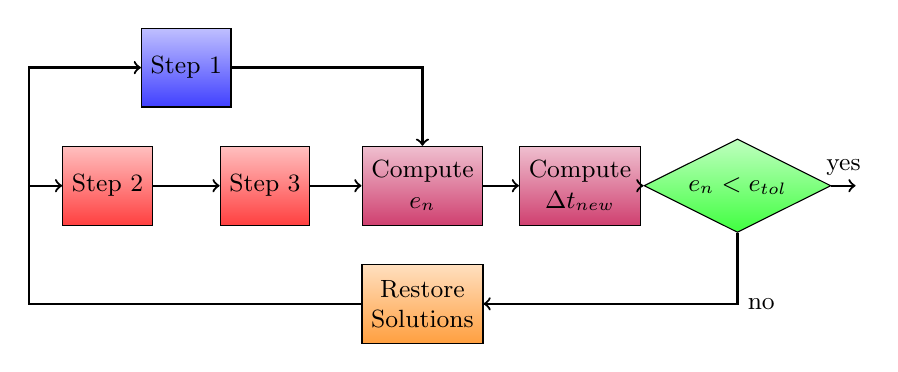
\begin{tikzpicture}[every node/.style = {font=\small},scale=0.5]

\node[blueblock](p1) at (-6,3) {Step 1} ;
\node[redblock](p2) at (-8,0) {Step 2} ;
\node[redblock](p3) at (-4,0) {Step 3} ;
\node[purpleblock](p4) at (0,0) {Compute \\ $e_n$};
\node[purpleblock](p5) at (4,0) {Compute  \\ $\Delta t_{new}$};
\node[greendiamond](p6) at (8,0) {$e_n < e_{tol}$};
\node[orangeblock](p7) at (0,-3) {Restore \\ Solutions};

\draw[->,thick](p1.east) -| (p4.north);
\draw[->,thick](p2.east) -- (p3.west);
\draw[->,thick](p3.east) -- (p4.west);
\draw[->,thick](p4.east) -- (p5.west);
\draw[->,thick](p5.east) -- (p6.west);
\draw[->,thick](p6.south) |- node[right] {no} (p7.east);
\draw[->,thick](p6.east) -- node[above] {yes} (11,0);
\draw[->,thick](p7.west) -| (-10,0) -- (p2.west);
\draw[->,thick](p7.west) -| (-10,0) |- (p1.west);

\end{tikzpicture}
\end{figure}
Each Step undergoes:
\bi
\item Shape evaluation
\item PRKE evaluations
\item Multiphysics evaluations
\item Iterations for convergence of amplitude, shape, and multiphysics
\ei



\end{block}

\end{frame}
%-------------------------------------------------------------------


%%%%%%%%%%%%%%%%%%%%%%%%%%%%%%%%%%%%%%%%%%%%%%%%%%%%%%%%%%%%%%%%%%%%
%%%%%%%%%%%%%%%%%%%%%%%%%%%%%%%%%%%%%%%%%%%%%%%%%%%%%%%%%%%%%%%%%%%%
\section{Results}
%%%%%%%%%%%%%%%%%%%%%%%%%%%%%%%%%%%%%%%%%%%%%%%%%%%%%%%%%%%%%%%%%%%%
%%%%%%%%%%%%%%%%%%%%%%%%%%%%%%%%%%%%%%%%%%%%%%%%%%%%%%%%%%%%%%%%%%%%

\subsection{TWIGL}

%-------------------------------------------------------------------
\begin{frame}{TWIGL Benchmark}
\begin{figure}
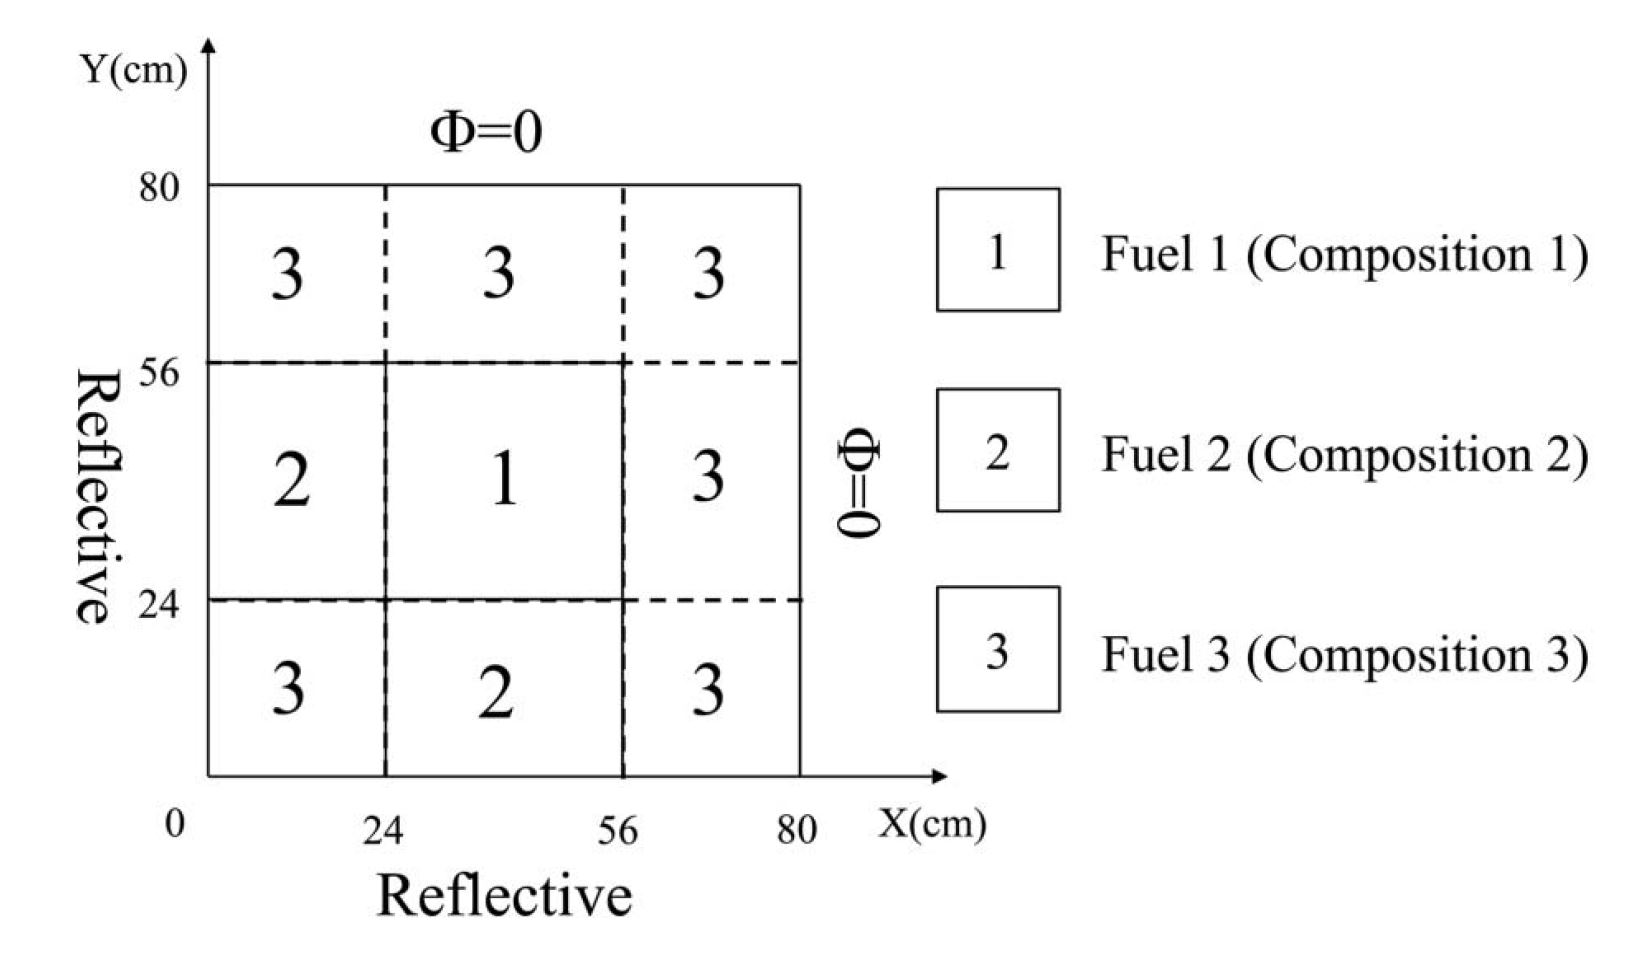
\includegraphics[width=\linewidth]{figures/TWIGL_regions.jpg}
\end{figure}
\end{frame}
%-------------------------------------------------------------------

%-------------------------------------------------------------------
\begin{frame}{TWIGL Results}

\begin{columns}

\column{.7\textwidth}
\begin{figure}
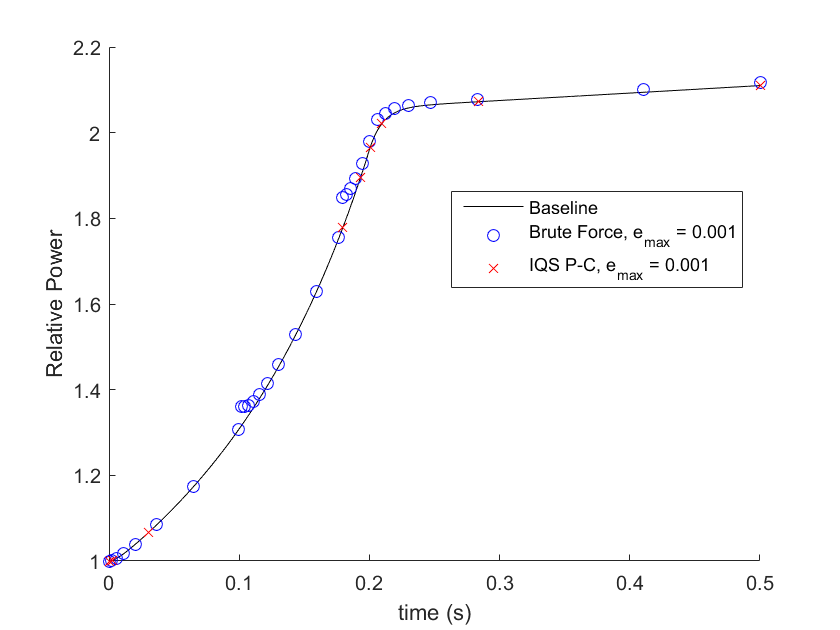
\includegraphics[width=\linewidth]{figures/TWIGL_power_plot.png}
\end{figure}

\column{.4\textwidth}
\begin{table}
\begin{center}
\resizebox{\textwidth}{!}{
\begin{tabular}{|l|l|l|l|l|}
\hline
\multicolumn{5}{|c|}{Brute Force}\\
\hline
Test & $e_{max}$ & Error & Steps & Solves \\
\hline
1 &	0.05    &	0.00012677 &	9    &	29 \\
2 &	0.01    &	3.5555e-05 &	11   &	35 \\
3 &	0.005   &	4.0364e-05 &	11   &	31  \\
4 &	0.001   &	0.00294822 &	33   &	122  \\
5 &	0.0005  &	0.00099778 &	39   &	131  \\
6 &	0.0001  &	0.00019510 &	78   &	236  \\
7 &	5.0e-05 &	0.00018372 &	112  &	342  \\
8 &	1.0e-05 &	8.0564e-05 &	263  &	794 \\
\hline

\end{tabular}}
\end{center}
\end{table}

\begin{table}
\begin{center}
\resizebox{\textwidth}{!}{
\begin{tabular}{|l|l|l|l|l|}
\hline
\multicolumn{5}{|c|}{IQS P-C} \\
\hline
Test & $e_{max}$ & Error & Steps & Solves \\
\hline
1 &	0.05    &	0.03380433 &	4  &	9   \\
2 &	0.01    &	0.00263068 &	5  &	12  \\
3 &	0.005   &	0.00160486 &	6  &	21  \\
4 &	0.001   &	1.7527e-05 &	10 &	35  \\
5 &	0.0005  &	1.4185e-05 &	16 &	74  \\
6 &	0.0001  &	6.2903e-06 &	19 &	78  \\
7 &	5.0e-05 &	1.5247e-06 &	24 &	92  \\
8 &	1.0e-05  &	9.8321e-07 &	48 &	210 \\
\hline
\end{tabular}}
\end{center}
\end{table}

\end{columns}

\end{frame}
%-------------------------------------------------------------------

\subsection{LRA}


%-------------------------------------------------------------------
\begin{frame}{LRA Benchmark}

\begin{figure}[h]
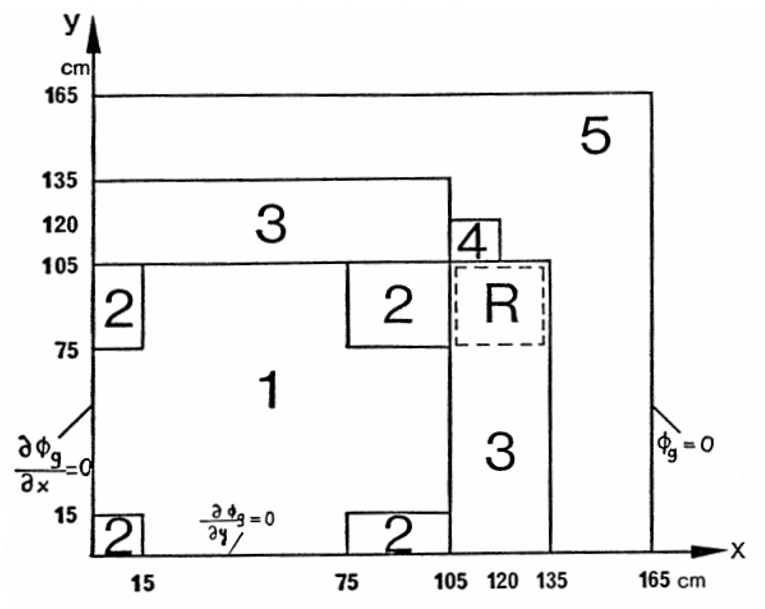
\includegraphics[height=0.8\textheight]{figures/lra_geom.png}
\end{figure}

\end{frame}
%-------------------------------------------------------------------

%-------------------------------------------------------------------
\begin{frame}{LRA Results}

\begin{columns}

\column{.58\textwidth}
\begin{figure}
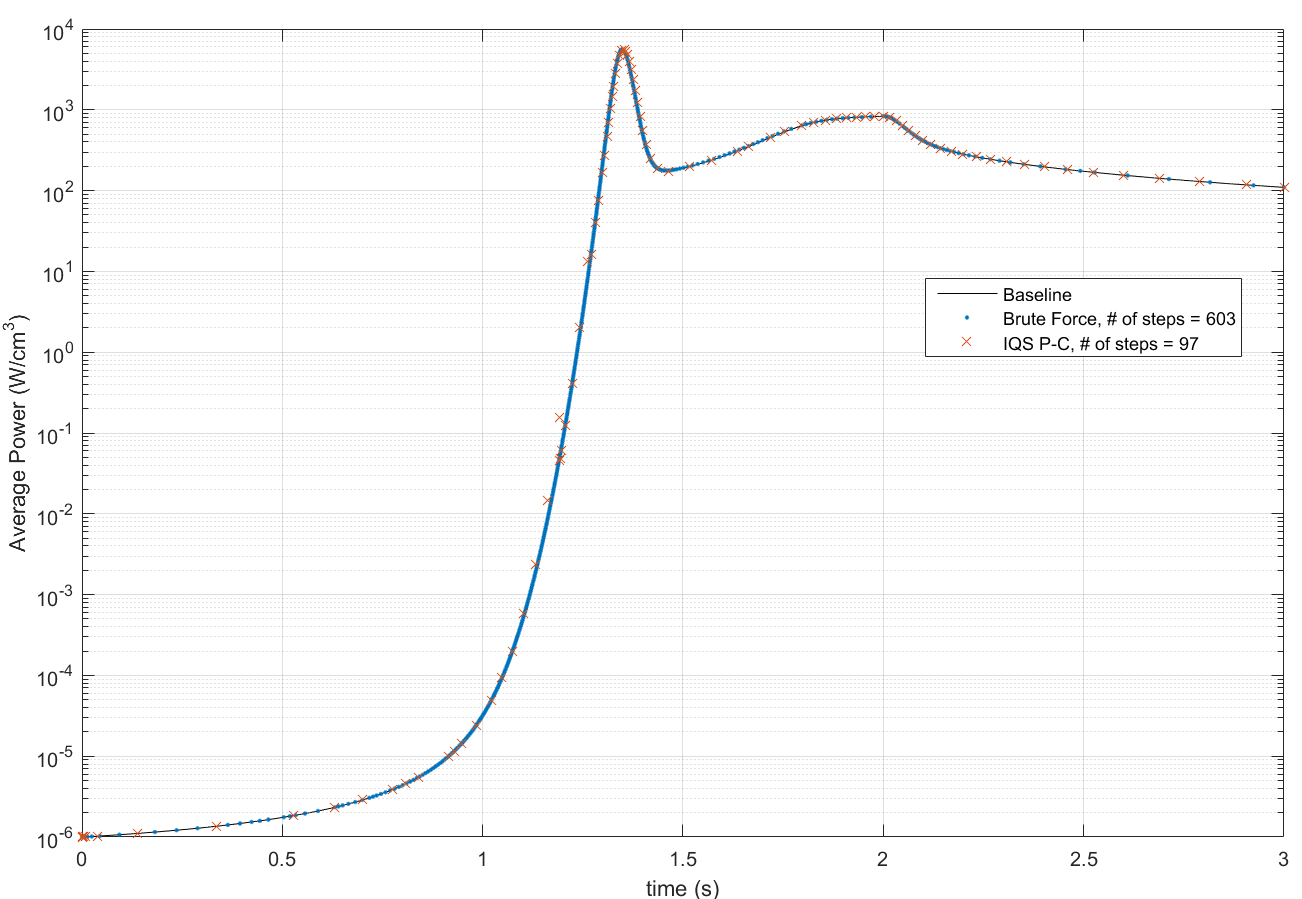
\includegraphics[width=\linewidth]{figures/LRA_DT2.png}
\end{figure}

\column{.58\textwidth}
\begin{figure}
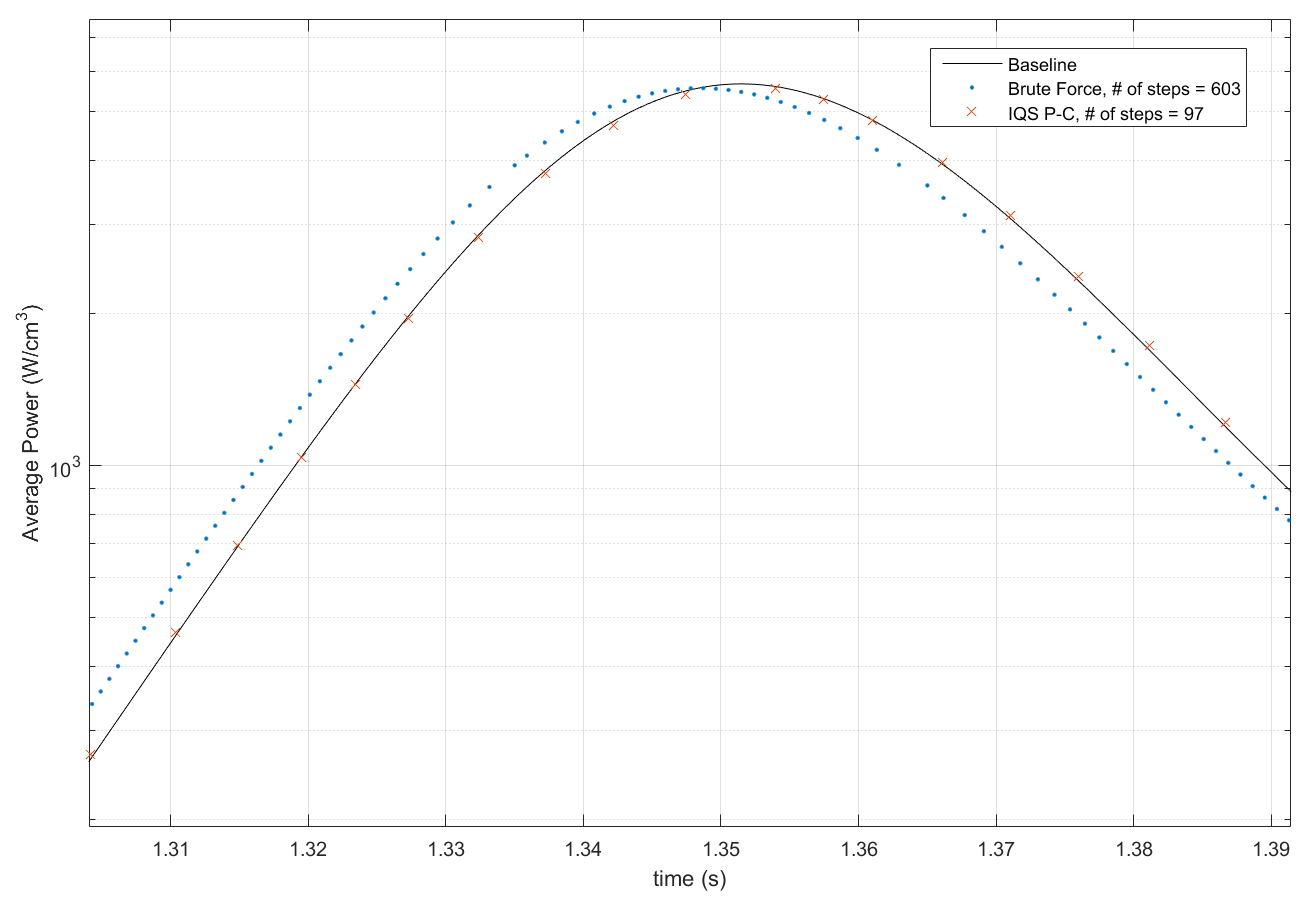
\includegraphics[width=\linewidth]{figures/LRA_DT2_peak.png}
\end{figure}

\end{columns}

\begin{table}
\begin{center}
\resizebox{\textwidth}{!}{
\begin{tabular}{|l|l|l|l|l|l|l|}
\hline
 & \multicolumn{3}{|c|}{Brute Force} & \multicolumn{3}{|c|}{IQS P-C} \\
\hline
Event & Power (W/cm$^3$) & Error & Steps & Power (W/cm$^3$) & Error & Steps \\
\hline
Max Power & 5567.3 & 0.019454 & 423 & 5568.3 & 0.019274 & 47 \\
End (3 s) & 109.66 & 2.3650e-4 & 603 & 109.65 & 3.0622e-4 & 97 \\
\hline
\end{tabular}}
\end{center}
\end{table}

\end{frame}
%-------------------------------------------------------------------


%%%%%%%%%%%%%%%%%%%%%%%%%%%%%%%%%%%%%%%%%%%%%%%%%%%%%%%%%%%%%%%%%%%%%
%%%%%%%%%%%%%%%%%%%%%%%%%%%%%%%%%%%%%%%%%%%%%%%%%%%%%%%%%%%%%%%%%%%%%
\section{Wrap-up}
%%%%%%%%%%%%%%%%%%%%%%%%%%%%%%%%%%%%%%%%%%%%%%%%%%%%%%%%%%%%%%%%%%%%%
%%%%%%%%%%%%%%%%%%%%%%%%%%%%%%%%%%%%%%%%%%%%%%%%%%%%%%%%%%%%%%%%%%%%%

%-------------------------------------------------------------------
\begin{frame}{Conclusion and Outlook}

\begin{block}{Completed}
\bi
\item Application and verification of step doubling IQS for pure neutronics
\item Application of step doubling IQS with simple temperature feedback
\ei
\end{block}

\begin{block}{In progress}
\bi 
\item Verification of IQS with temperature feedback
\item Exploration of IQS techniques for multiphysics feedback
\item Application of step doubling IQS for full core TREAT model
\ei
\end{block}

\begin{block}{Next Steps}
\bi 
\item Implementation of IQS into Newton iteration process
\item IQS application to SAAF-S$_N$ and transport benchmarks
\ei
\end{block}

\end{frame}
%-------------------------------------------------------------------

%-------------------------------------------------------------------
\begin{frame}{Questions ?}


\begin{block}{Thank you}
\begin{itemize}
\item Yaqi Wang (INL, Rattlesnake lead)
\item Mark DeHart (INL, TREAT M\&S lead)
\item NEAMS
\end{itemize}
\end{block}

\end{frame}
%-------------------------------------------------------------------


%%-------------------------------------------------------------------
%\begin{frame}{}
%
%
%\begin{block}{}
%\end{block}
%
%\end{frame}
%%-------------------------------------------------------------------

%%%%%%%%%%%%%%%%%%%%%%%%%%%%%%%%%%%%%%%%%%%%%%%%%%%%%%%%%%%%%%%%%%%%
%%%%%%%%%%%%%%%%%%%%%%%%%%%%%%%%%%%%%%%%%%%%%%%%%%%%%%%%%%%%%%%%%%%%
%\begin{frame}{Thank you}
%
%\begin{block}{Computational Transport}
%\begin{figure}
%	\centering
%	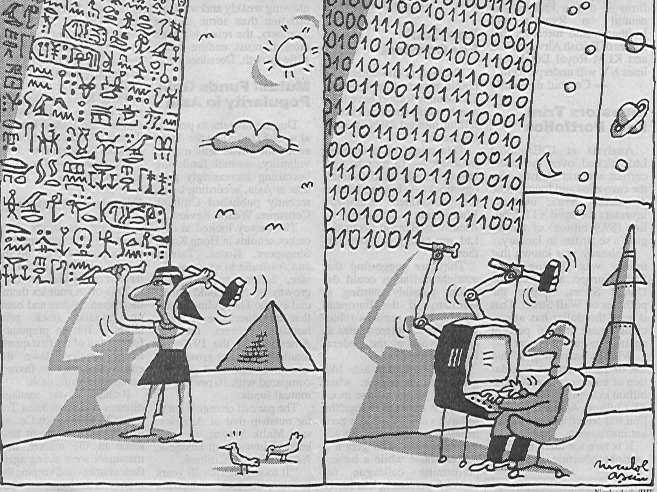
\includegraphics[scale=0.33]{./fig/crunching.png}
%\end{figure}
%\end{block}
%
%\end{frame}
%%%%%%%%%%%%%%%%%%%%%%%%%%%%%%%%%%%%%%%%%%%%%%%%%%%%%%%%%%%%%%%%%%%%
%%%%%%%%%%%%%%%%%%%%%%%%%%%%%%%%%%%%%%%%%%%%%%%%%%%%%%%%%%%%%%%%%%%%

%************************************************

\end{document}